\begin{song}{title=\predtitle \centering John Brown \\\large  }  %% sem se napíše jméno songu a autor


\vetsi

\moveleft 0.6cm \vbox{

\begin{centerjustified}
\begin{varwidth}[t]{0.5\textwidth}\setlength{\parindent}{\pindent}  %Varianta č. 2 --> Dva sloupce

\vspace*{-0.43cm}
\sloka
^{G\z}Černý muž pod bičem otrokáře žil,

^{C\z}černý muž pod bičem ^{G\z}otrokáře žil,

černý muž pod bičem otrokáře ^{Emi\z}žil,~~~

^{\z \z A7}kapitán John ^{D7\z}Brown to ^{G\z}zřel.

\refren
^{G\z}Glory, glory, haleluja,

^{C\z}glory, glory, ^{G}haleluja,

glory, glory, ^{\z Emi}haleluja,

^{\z Ami}kapitán John ^{D7\z}Brown to ^{G\z}zřel.

\sloka
/: Sebral z Virginie černých přátel

šik, :/

sebral z Virginie černých přátel šik,

prapor svobody pak zdvih'.

\refren
\dots  prapor svobody pak zdvih'.

\end{varwidth}\mezisloupci\begin{varwidth}[t]{0.55\textwidth}\setlength{\parindent}{\pindent}
\vspace*{0.03cm}

\sloka
/: V čele věrných město Harper's Ferry

jal, :/

v čele věrných město Harper's Ferry jal,

právo vítězí a čest.

\refren
\dots  právo vítězí a čest.



\sloka
/: Hrstka statečných však udolána jest,\,:/

hrstka statečných však udolána jest,

kapitán John Brown je jat.

\refren
\dots  kapitán John Brown je jat.



\sloka
^{}/:\,Zvony\,Charlestonu\,z\,dáli\,temně\,zní,\,:/

zvony Charlestonu z dáli temně zní,

Johnův den to poslední.

\refren
\dots  Johnův den to poslední.

\sloka
/:\,John\,Brown\,mrtev\,jest\,a\,jeho\,tělo\,tlí,\,:/

John Brown mrtev jest a jeho tělo tlí,

jeho duch však kráčí dál.

\refren
\dots  jeho duch však kráčí dál.

\end{varwidth}
\end{centerjustified}

\hrulefill

\begin{minipage}{\textwidth}

\begin{wrapfigure}{R}{0.25\textwidth}
\centering
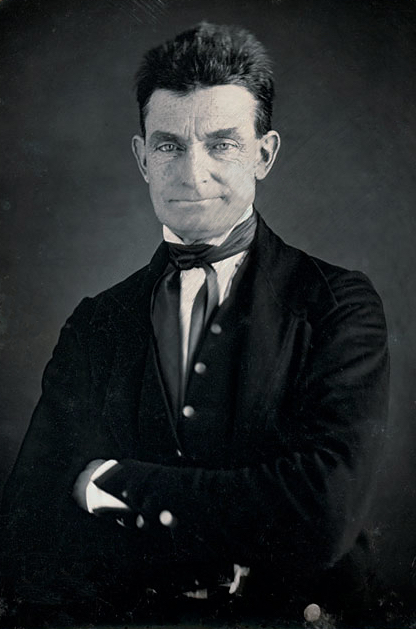
\includegraphics[width=0.23\textwidth]{../img/JohnBrown.jpg}
\end{wrapfigure}

\begin{small}
V~odbobí cca od 17. do 19. století se mezi Evropou, Afrikou a Amerikou vytvořil
tzv. trojúhelníkový obchod. Evropské lodě vyplouvaly s nákladem textilu rumu a~jiných
výrobků sestavených v Evropě do Afriky, kde je vyměnili za \textbf{otroky}.
Evropští kolonizátoři totiž nejen dobývali země patřící obyvatelům Afriky, ale samotným Afričanům
odmítli přiznat lidskost tím, že je považovali na pouhé věci, které se daly prodávat.
Ačkoliv Afričané vzdorovali \footnote{\url{https://slaveryandremembrance.org/articles/article/?id=A0035}}
v~nelidských podmínkách (úmrtnost na lodích byla průměrně 15 \%), je Evropani dovezli do
USA, kde je vyměnili za cukr, tabák a bavlnu, kterou dovezli zpět do Evropy.

Život otroka*yně po vylodění v USA však nebyl o nic lehčí než cesta vzhledem
k~tomu, že otroci neměli skoro žádná práva. Na denním pořádku bylo např.
znásilňování, fyzické tresty (či rovnou mučení) a~nucená práce. Vlastnění
otroků bylo přitom normou, např. první prezident USA G. Washington také vlastnil
otroky.

Ne všichni bílí Američané to ale považovali za správné, ti, kteří chtěli
otroctví zrušit, si říkali abolicionisté. O jednom z nich jménem John Brown
a jeho ozbrojeném pokusu osvobodit otroky tato píseň zpívá.

Otroctví bylo v USA zakázáno r. 1865.
I~dnes otroctví v~jistých částech světa přetrvává.
Afroameričané však stále v~USA čelí systémovému rasismu.
Např. v~r. 2022 je v~tamních vězeních celkem 2 miliony lidí, z toho 38 \% Afr.,
i~když tvoří jen 12 \% populace.
\end{small}
\end{minipage}
}

\setcounter{Slokočet}{0}
\end{song}

